\documentclass[PI,LAB]{HSEUniversity}

\usepackage{graphicx}
\graphicspath{ {img/} }

\usepackage{hyperref}
\hypersetup{
    colorlinks=true,
    linkcolor=black,
    filecolor=magenta,      
    urlcolor=cyan,
}

\title{Организация паттернов проектирования. Порождающий паттерн <<Строитель>>}
\author{Рязанов Иван Дмитриевич}
\supervisor{к.т.н., доцент кафедры Информационных технологий в бизнесе НИУ ВШЭ-Пермь}{А.В.~Кычкин}
\Year{2020}

\begin{document}
\maketitle
\chapter{Паттерн <<Строитель>>}
\textbf{Название и классификация паттерна.}
Строитель - паттерн, порождающий объекты.

\textbf{Назначение.}
Отделяет конструирование сложного объекта от его представления, так что в результате одного и того же процесса конструирования могут получаться разные представления.
В паттерне строитель абстрагированы все эти отношения. В нем любой класс конвертора называется строителем, а загрузчик – распорядителем.

\textbf{Применимость.}
Использование паттерна Строитель целесообразно если:
\begin{itemize}
  \item процесс создания нового объекта не должен зависеть от того, из каких частей этот объект состоит и как эти части связаны между собой;
  \item необходимо обеспечить получение различных вариаций объекта в процессе его создания.
\end{itemize}
\clearpage

\begin{figure}[p]
  \centering
  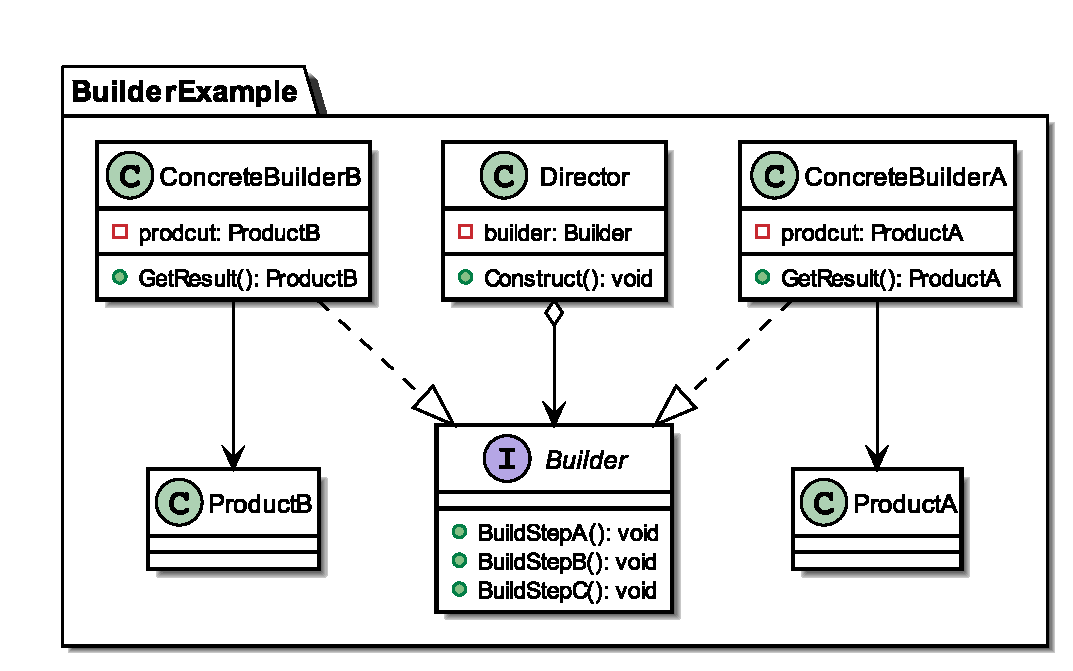
\includegraphics[scale=0.7]{Builder_CD.eps}
  \caption{Диаграмма классов паттерна <<Строитель>>}
\end{figure}

\begin{figure}[p]
  \centering
  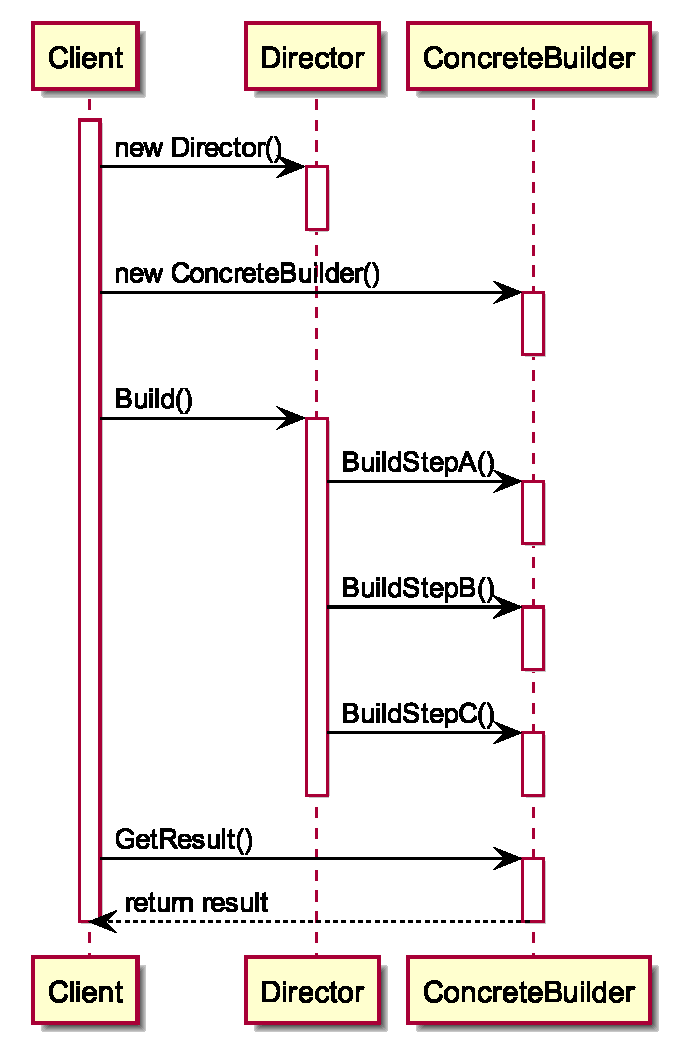
\includegraphics[scale=0.75]{Builder_SD.eps}
  \caption{Диаграмма последовательности паттерна <<Строитель>>}
\end{figure}
\clearpage

\textbf{Участники}
\begin{itemize}
  \item Builder - абстрактный строитель: объявляет интерфейс для операций, создающих части продукта;
  \item ConcreteBuilder (ConcreteBuilderA, ConcreteBuilderB) - конкретный строитель: реализует операции, создающие конкретные части продукта;
  \item Product (ProductА, ProductВ) - продукт: определяет объект-продукт, создаваемый соответствующим строителем;
  \item Director - распорядитель (директор): пошагово конструирует продукт, используя методы строителя;
\end{itemize}

\textbf{Отношения}
\begin{itemize}
  \item клиент создает объект-распорядитель Director и конфигурирует его нужным объектом-строителем Builder;
  \item распорядитель уведомляет строителя о том, что нужно построить очередную часть продукта;
  \item строитель обрабатывает запросы распорядителя и добавляет новые части к продукту;
  \item клиент забирает продукт у строителя.  
\end{itemize}

\textbf{Плюсы и минусы}

Плюсы:
\begin{itemize}
   \item возможность контролировать процесс создания сложного продукта;
   \item возможность получения разных представлений некоторых данных. 
  \end{itemize}

Минусы:
\begin{itemize}
  \item ConcreteBuilder и создаваемый им продукт жестко связаны между собой, поэтому при внесении изменений в класс продукта скорее всего придется соответствующим образом изменять и класс ConcreteBuilder. 
\end{itemize}
\clearpage

\textbf{Области применения}

\begin{enumerate}
  \item Создание XML-документов или HTML-документов с помощью классов-строителей с методами для создания элементов документа (тегов).
  \item Класс StringBuilder в C\verb|#|.
\end{enumerate}

\chapter{Проектирование и реализация}
\section{Проектирование}
Для реализации был выбран 1 вариант:

<<Создание отчета, содержащего различные графические компоненты (текст, диаграммы, графики), которые могут идти в произвольном порядке.>>

Перед началом работы построим диаграмму классов (см. рис. \ref{fig:Task_CD}).
 \begin{figure}[p]
   \centering
   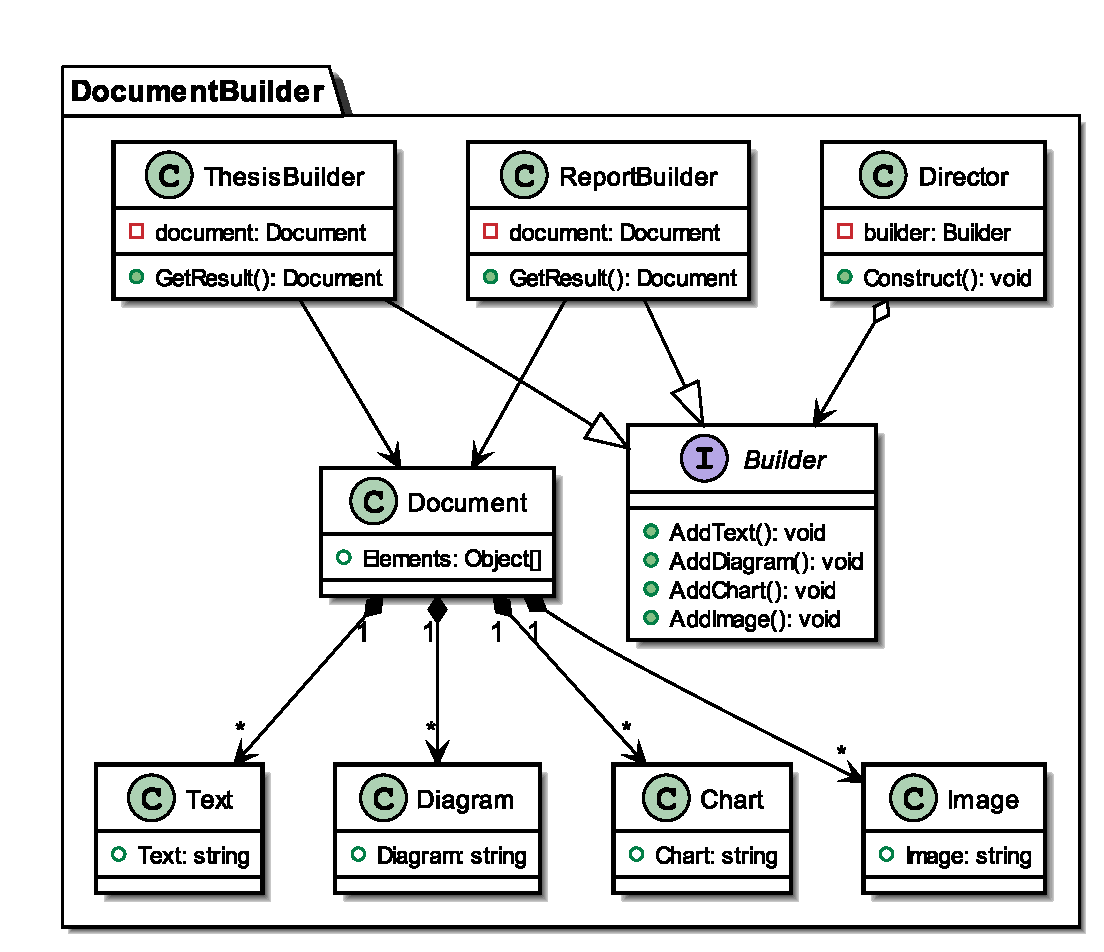
\includegraphics[scale=0.75]{Task_CD.eps}
   \caption{Диаграмма классов}
   \label{fig:Task_CD}
 \end{figure}

\textbf{Участники}
\begin{itemize}
  \item Builder - абстрактный строитель: объявляет интерфейс для операций, создающих части продукта;
  \item ThesisBuilder, ReportBuilder - конкретные строители: реализуют операции, создающие разные типы документов (Курсовая или отчет);
  \item Document - продукт: документ, создаваемый соответствующим строителем;
  \item Director - распорядитель (директор): пошагово конструирует продукт, используя методы строителя;
  \item Text - текст;
  \item Diagram - диаграмма;
  \item Chart - график;
  \item Image - изображение.
\end{itemize}

\section{Реализация}
Реализация паттерна <<Строитель>> находится в git-репозитории по ссылке: \href{https://github.com/rovany706/design-patterns/tree/master/Builder/src/com/Builder}{github.com}

\end{document}